\section{Experimental setup and results}
In this section the experimental setup is described and the 
results of three experiments are presented.
In the first one the robot is supposed to press an emergency button with variables
force references. In the second and in the third one the robot drags an object on a table 
while the contact force is regulated until 
it reaches the edge of the table and sticks out of it.

\subsection{Experimental setup}
The test-bed for this project is a Kuka LWR$4+$, a $7$-joints industrial manipulator, 
which is provided with an internal software layer called Fast Research Interface (FRI).
\begin{figure}[h]
  \centering
  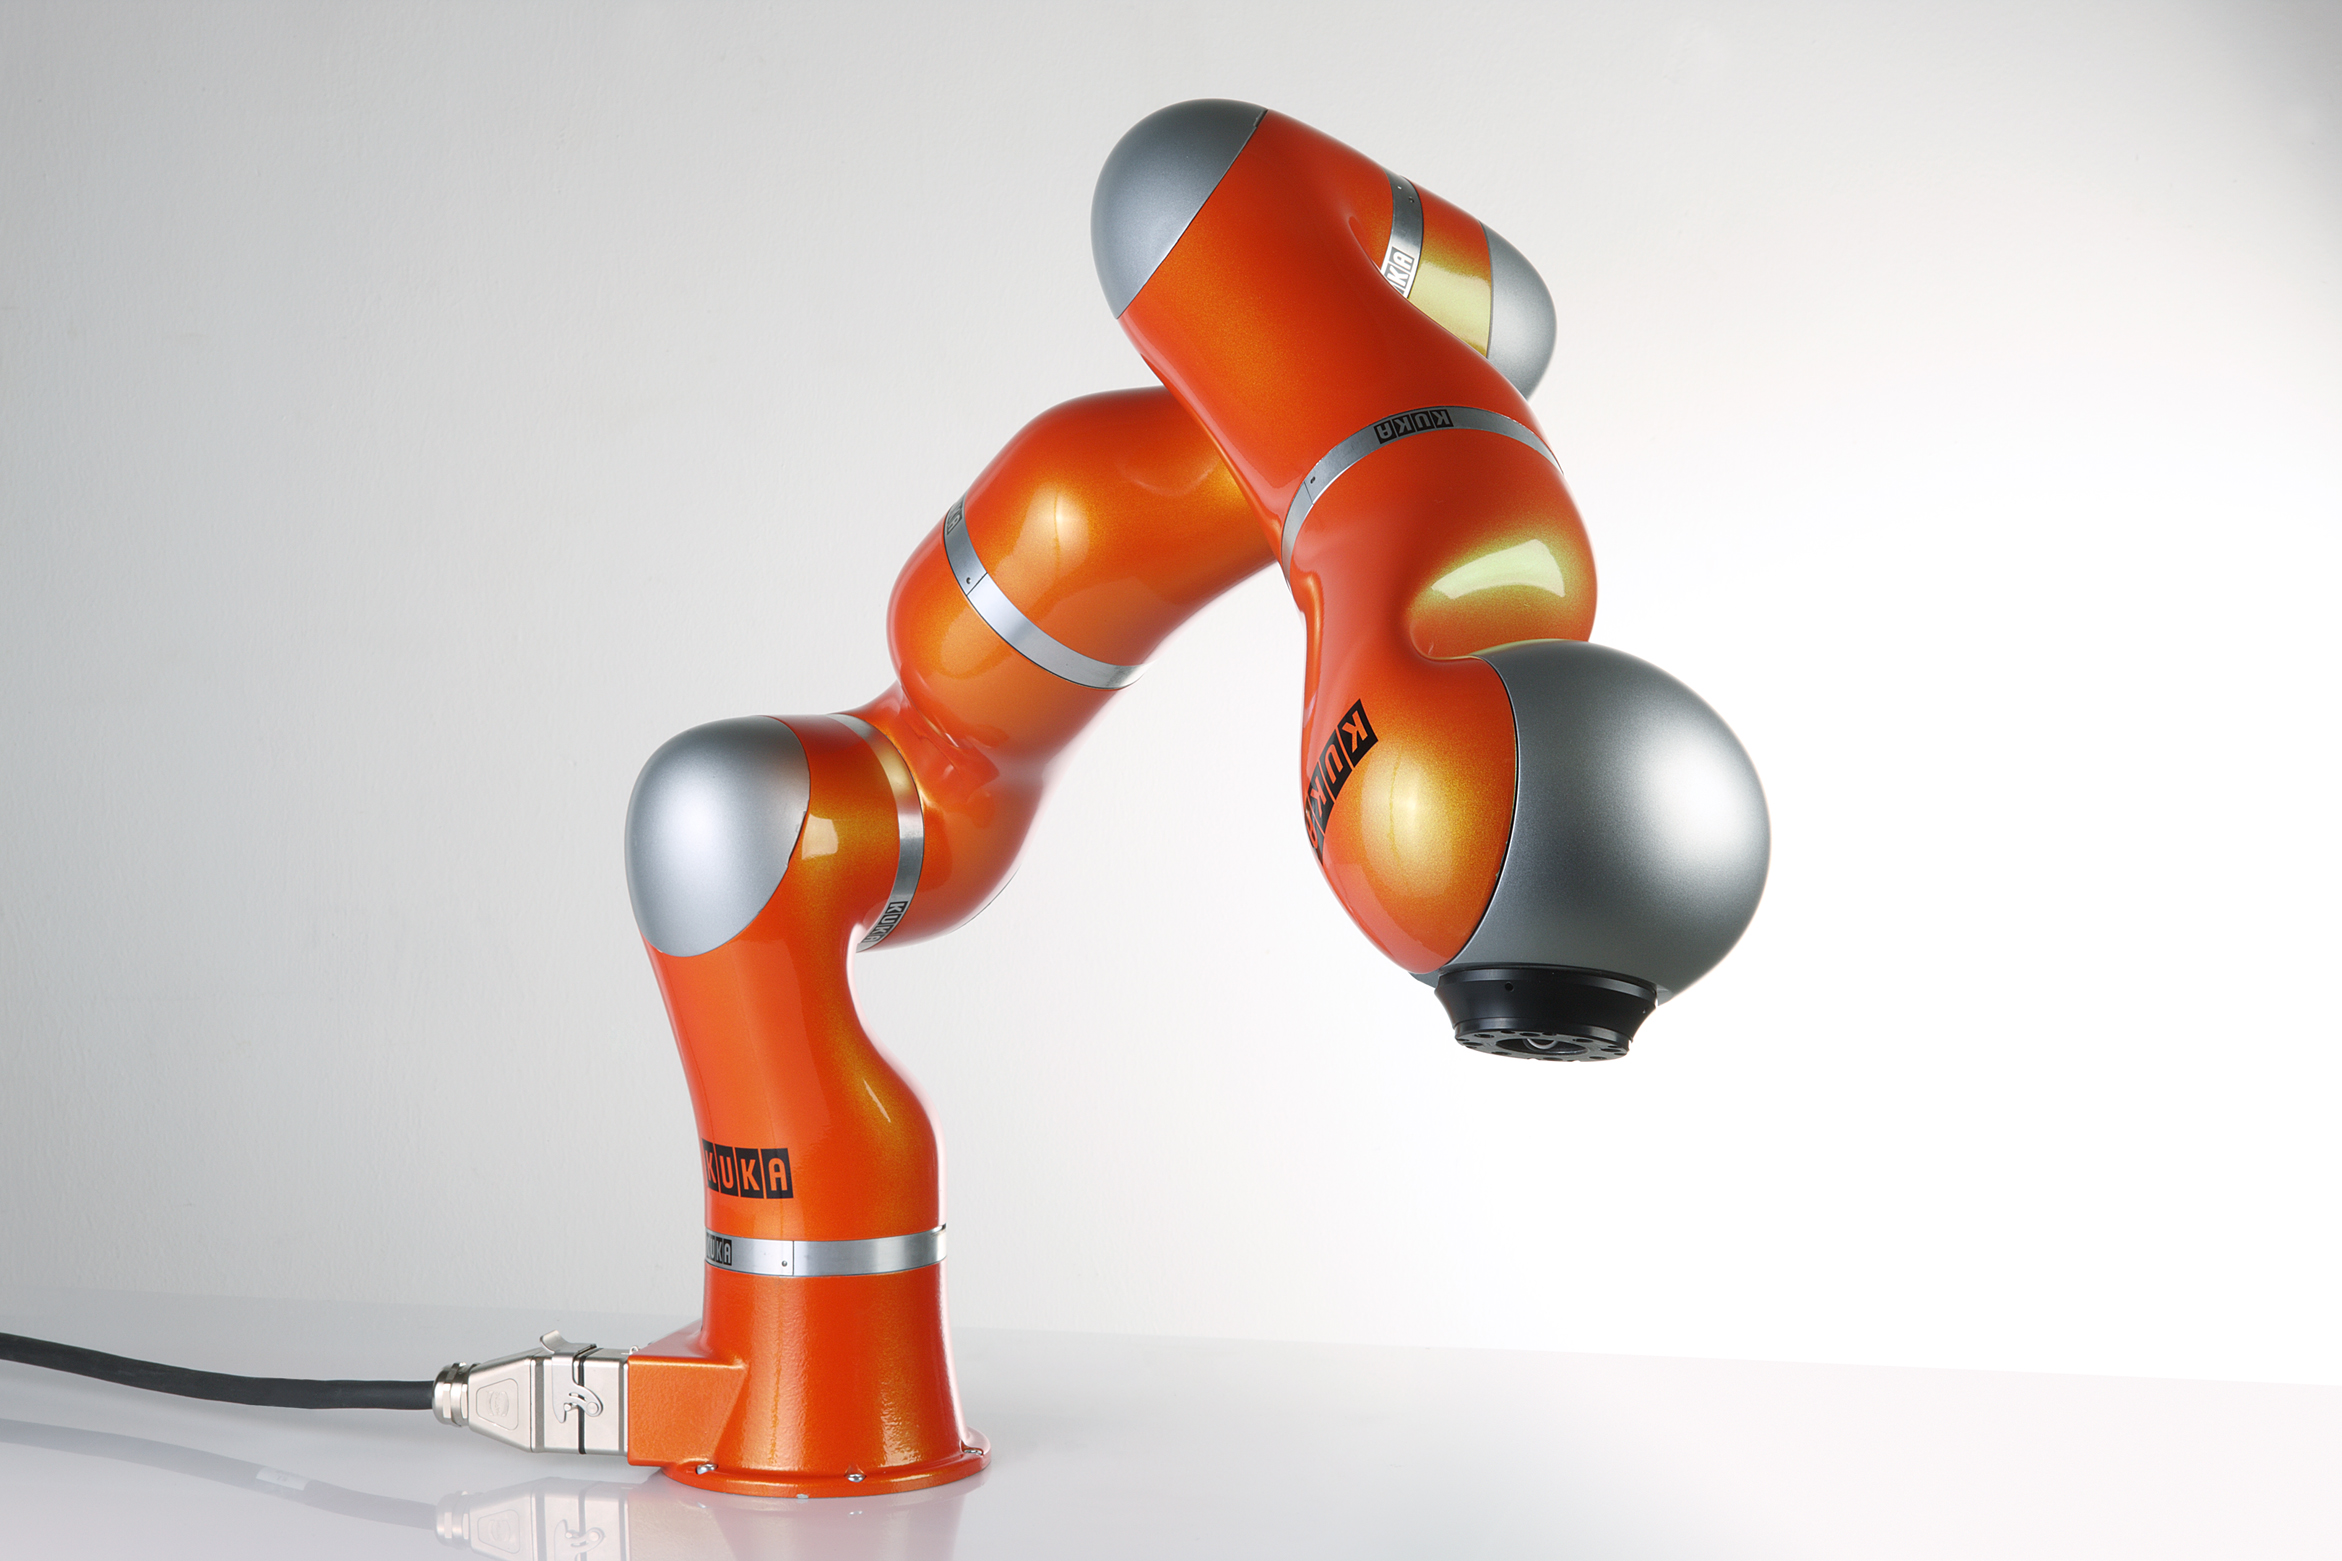
\includegraphics[scale=0.5]{KUKA.jpg}
  \caption{KUKA LWR$4+$ manipulator. \label{fig:kuka_lwr}}
\end{figure}
\par
In order to send the control laws, described in the previous sections, to the robot
 one of the internal modes of operation, called Joints Specific Impedance, was used
\[
\boldsymbol{\tau}_{cmd} = K_j(\vec{q}_{FRI} - \vec{q}_{msr}) + D(d_{j}) + \boldsymbol{\tau}_{FRI} + \vec{f}_{dynamics}(\vec{q}, \dot{\vec{q}}, \ddot{\vec{q}})
\]
where $\boldsymbol{\tau}_{cmd}$ is the effective torque sent to the robot, 
$\vec{q}_{FRI}$ is the vector of the desired angular positions of the joints, 
$\vec{q}_{msr}$ is the vector of the angular positions of the joints, 
$K_j$ and $D(d_j)$ are gains that shape the dynamics of the impedance control mode,
$\boldsymbol{\tau}_{FRI}$ is an additional torque provided by the user and 
$\vec{f}_{dynamics}(\vec{q}, \dot{\vec{q}}, \ddot{\vec{q}})$ is a gravity compensation
term provided by the producer.
\par
Since the control laws developed are pure torque laws only the term
$\boldsymbol{\tau}_{FRI}$ was used and the others were set as:
\begin{itemize}
\item[-] $K_j = 0$;
\item[-] $d_j = 0$;
\item[-] $\vec{q}_{FRI} = \vec{q}_{msr}$
\end{itemize}

\subsubsection{Force Torque sensor}
The force/torque sensor used in this work is an ATI Mini$45$
\cite{ATIIndustrialAutomation2017}.
In all the experiments the measured signal was filtered using a built-in
LP filter with cutoff frequency of $\SI{8}{Hz}$.

\subsubsection{Notes about controllers implementation}
In order to implement the control laws
\[
\begin{split}
  \vec{\tau} &= C \dot{\vec{q}} + B \vec{a}_{p2p}\\
  \vec{\tau} &= C \dot{\vec{q}} + {}^{b}J^{T}_{F} ( \Lambda_A \vec{a}_{cmd} - \Lambda_A {}^{ws} \dot{J_{A,E}} \dot{\vec{q}} + {}^b\vec{w}_{F}) +
  (I_7 - ({}^{b}J^{T}_{F}) ({}^{b} \bar{J}^{T}_{F})) \vec{\gamma}_{0}
\end{split}
\]
several quantities are required among which
\begin{itemize}
\item[-] angular position, velocity and acceleration of the joints;
\item[-] Jacobians;
\item[-] inertia matrix;
\item[-] Coriolis matrix;
\item[-] direct and inverse kinematics facilities;
\item[-] Euler ZYZ kinematical matrix.
\end{itemize}
\par
The angular position are provided by the FRI software layer.
The angular velocities and the angular accelerations are not provided by
the producer so they were estimated using an exponential smoothing filter of the 
form
\[
\begin{cases}
  \dot{\vec{q}}_0 = \vec{0} \\
  \dot{\vec{q}}_k = (1 - \alpha) \dot{\vec{q}}_{k-1} + \alpha \frac{\vec{q}_k - \vec{q}_{k-1}}{t_s}
\end{cases}
\]
\[
\begin{cases}
  \ddot{\vec{q}}_0 = \vec{0} \\
  \ddot{\vec{q}}_k = (1 - \alpha) \ddot{\vec{q}}_{k-1} + \alpha \frac{\dot{\vec{q}}_k - \dot{\vec{q}}_{k-1}}{t_s}
\end{cases}
\]
where the constant $\alpha \in [0, 1]$ is the smoothing factor and $t_s$ is the sampling time.
In all the experiments $\alpha = 0.2$ and $t_s = \SI{3}{ms}$.
\par
All the others quantities were evaluated numerically using the facilities offered by the KDL library which was
integrated into the already existing KUKA LWR$4+$ software stack provided to the students

\subsection{Experiment 1}
In this experiment (fig. \ref{fig:hand_button}) the robot is supposed to press an emergency button.
\begin{figure}[h]
  \centering
  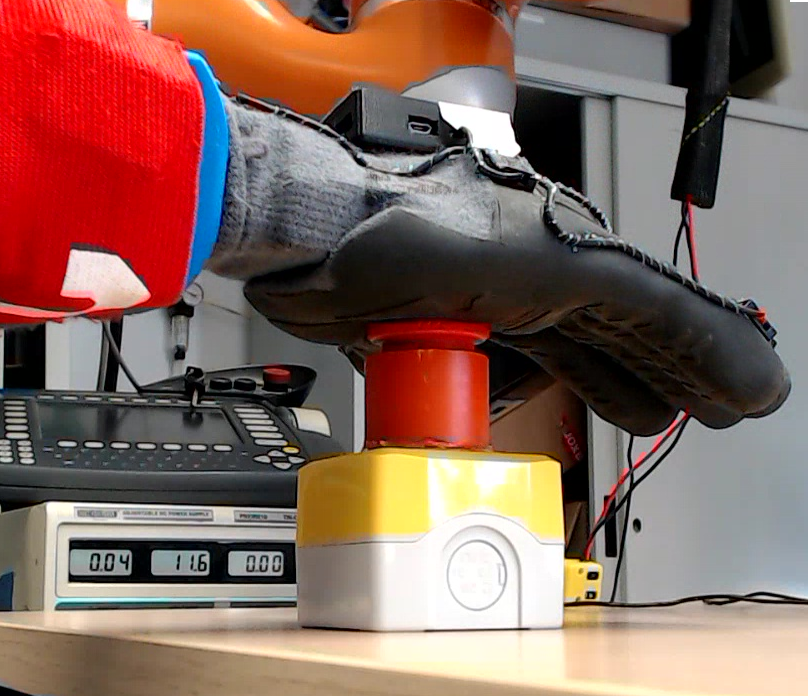
\includegraphics[scale=0.37]{hand_button.png}
  \caption{The hand while it presses the emergency button. \label{fig:hand_button}}
\end{figure}
\par
Initially a reference command of approximately $\SI{1}{N}$ is sent to the robot
until the contact takes place. Then several set points are sent to the robot:
\begin{itemize}
\item[-] $F_{z,des} = \SI{-2.5}{N}$
\item[-] $F_{z,des} =\SI{-1.5}{N}$
\item[-] $F_{z,des} =\SI{-3.5}{N}$
\item[-] $F_{z,des} =\SI{-1}{N}$
\end{itemize}
\par
The results, presented in the Table \ref{fig:button},
\begin{table}[h]
  \begin{tabular}{cc}
    \begin{subfigure}{0.5\textwidth}
      \centering
      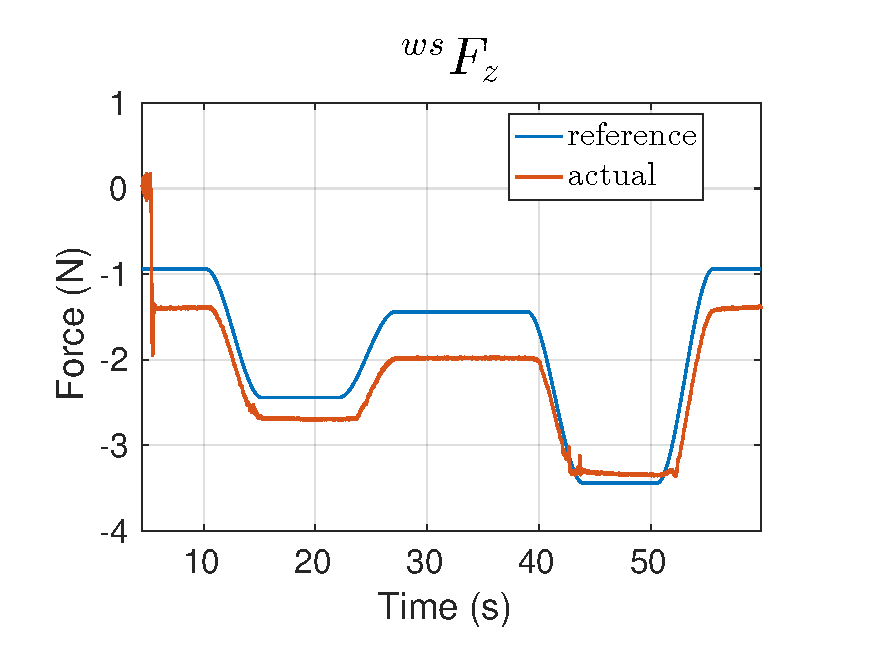
\includegraphics[scale=0.5]{button_z}
      \caption{Reference and actual force. \label{fig:button_z}}
    \end{subfigure}&
    \begin{subfigure}{0.5\textwidth}
      \centering
      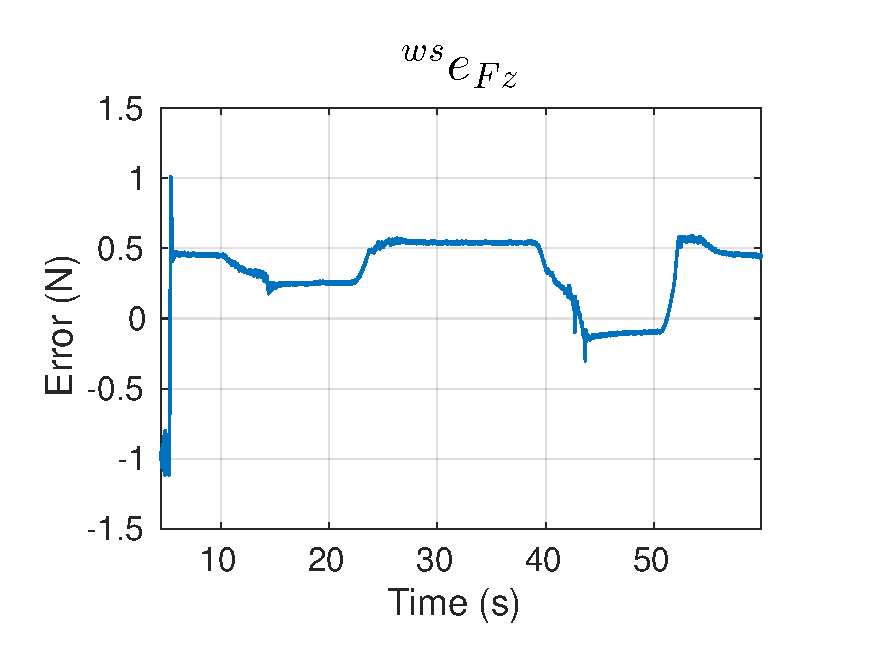
\includegraphics[scale=0.5]{button_err_z}
      \caption{Error. \label{fig:button_error_z}}
    \end{subfigure} 
  \end{tabular}
  \caption{Experiment 1, the hand presses a button.\\
  $K_f = 2$ and $B_f = 45$\label{fig:button}}
\end{table}
show that the error after the contact phase is bounded between
$\SI{-0.35}{N}$ and $\SI{0.5}{N}$ and it decreases as the requested force 
increases. The contact phase is visible as a spike in the measured force
(see Table \ref{fig:button_z}).

\subsection{Experiment 2}
In this experiment (Fig. \ref{fig:hand_banana}) a banana is dragged 
on a table while the contact force between the hand and the fruit is regulated.
\begin{figure}[h]
  \centering
  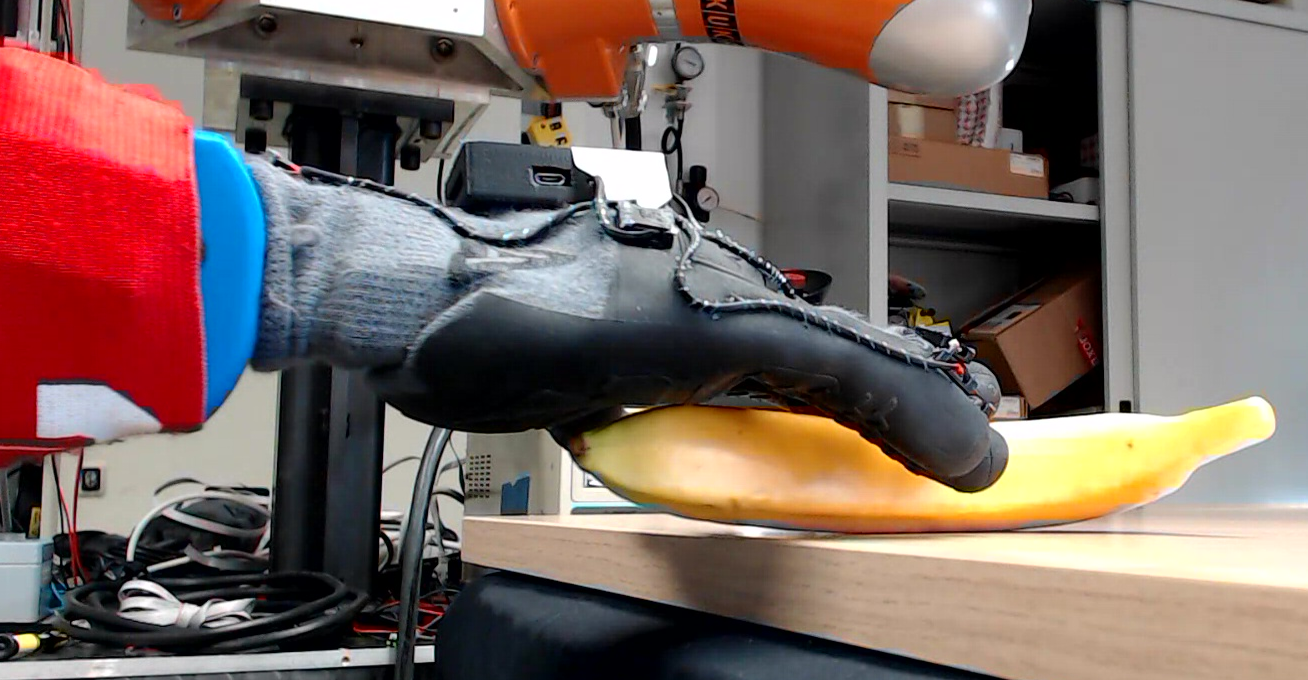
\includegraphics[scale=0.25]{hand_banana.png}
  \caption{The hand while it drags the banana. \label{fig:hand_banana}}
\end{figure}
The object is dragged in $\SI{5}{s}$ for a distance of $\SI{12}{cm}$ and the requested force is $\SI{3}{N}$.
In the Table \ref{fig:banana} only the results of the dragging phase are shown.
\begin{table}[h]
  \begin{tabular}{cc}
    \begin{subfigure}{0.5\textwidth}
      \centering
      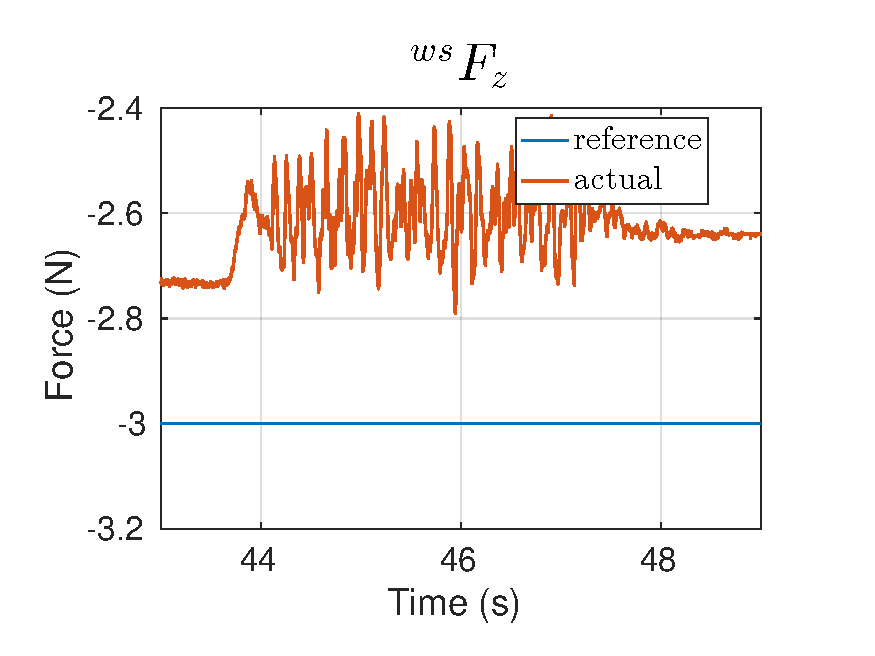
\includegraphics[scale=0.5]{banana_z}
      \caption{Reference and actual force. \label{fig:banana_z}}
    \end{subfigure}&
    \begin{subfigure}{0.5\textwidth}
      \centering
      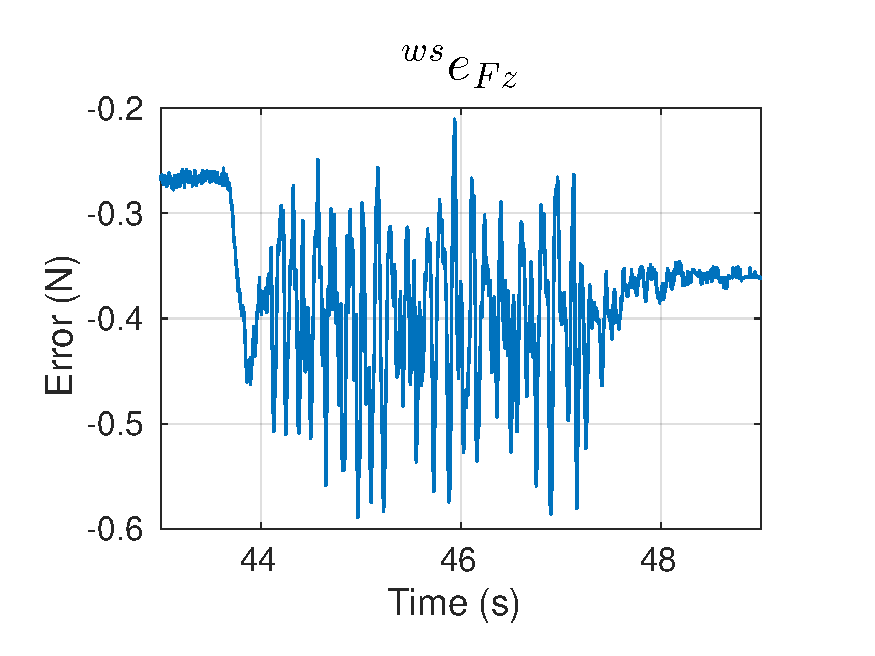
\includegraphics[scale=0.5]{banana_err_z}
      \caption{Error. \label{fig:banana_error_z}}
    \end{subfigure}\\
    \begin{subfigure}{0.5\textwidth}
      \centering
      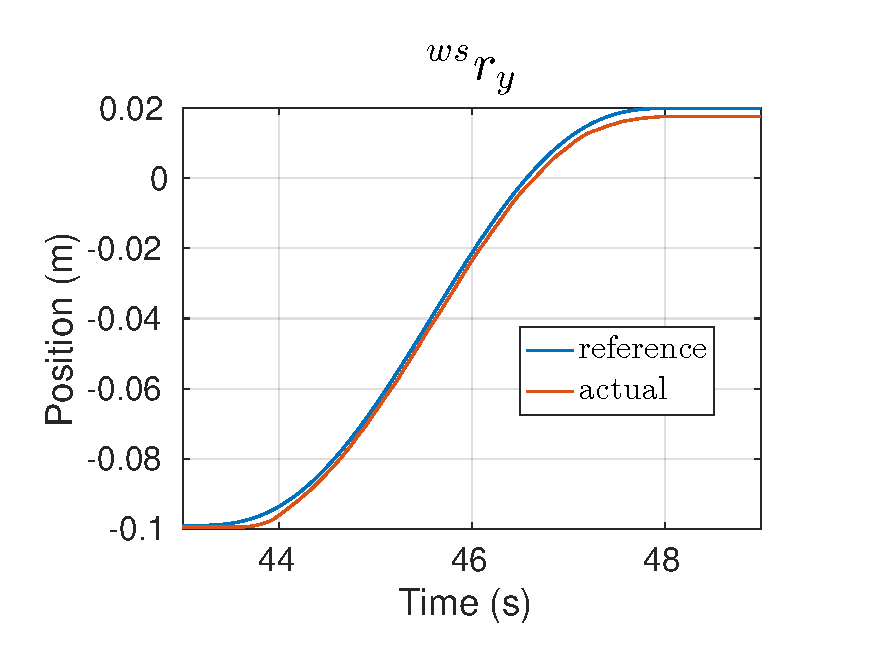
\includegraphics[scale=0.5]{banana_y}
      \caption{Reference and actual trajectory. \label{fig:banana_y}}
    \end{subfigure}&
    \begin{subfigure}{0.5\textwidth}
      \centering
      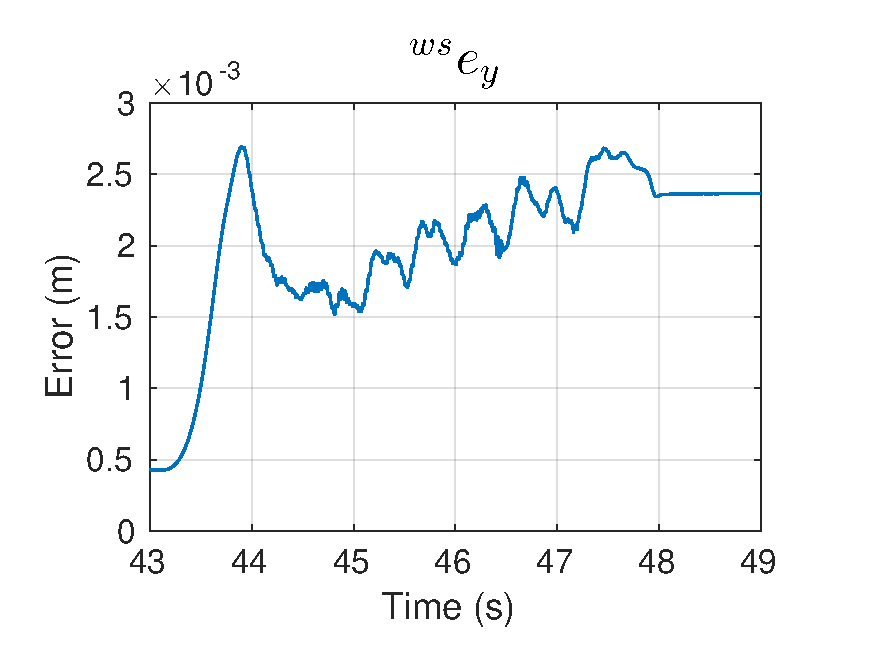
\includegraphics[scale=0.5]{banana_err_y}
      \caption{Error. \label{fig:banana_error_y}}
    \end{subfigure}
  \end{tabular}
  \caption{Experiment 2, the hand drags a banana.\\
  $K_f = 2.5$ and $B_f = 85$.}\label{fig:banana}
\end{table}
Although the force error is bounded between $\SI{-0.6}{N}$ and 
$\SI{-0.25}{N}$ undesired spikes are present because of
the vibrations due to the movement.

\subsection{Experiment 3}
\newpage
